\documentclass[12pt]{article}
\textwidth=17cm \oddsidemargin=-0.9cm \evensidemargin=-0.9cm
\textheight=23.7cm \topmargin=-1.7cm
\headheight=14.5pt

\usepackage{amssymb, amsmath, amsfonts}
\usepackage{moreverb}
\usepackage{graphicx}
\usepackage{enumerate}
\usepackage{graphics}
\usepackage{color}
\usepackage{array}
\usepackage{float}
\usepackage{hyperref}
\usepackage{textcomp}
\usepackage{alltt}
\usepackage{physics}
\usepackage{nicefrac}
\usepackage{mathtools}
\usepackage{tikz}
\usepackage{pgfplots}
\pgfplotsset{compat=1.13}
\usetikzlibrary{positioning}
\usetikzlibrary{arrows}
\usepackage{bigints}
\usepackage[utf8]{inputenc}
\usepackage[english]{babel}
\usepackage{amsthm}
\usepackage{fancyhdr}
\usepackage[makeroom]{cancel}
\pagestyle{fancy}
\allowdisplaybreaks

\newcommand{\E}{\varepsilon}

\newcommand{\suchthat}{\, \mid \,}
\newcommand{\ol}[1]{\overline{#1}}
\newcommand{\bbar}[1]{\overline{#1}}
\newcommand{\inpd}[1]{{\left< \, #1 \, \right>}}
\renewcommand{\theenumi}{\alph{enumi}}
\newcommand\Wider[2][3em]{%
\makebox[\linewidth][c]{%
  \begin{minipage}{\dimexpr\textwidth+#1\relax}
  \raggedright#2
  \end{minipage}%
  }%
}

\def\R{\mathbb{R}}
\def\C{\mathbb{C}}
\def\H{\mathcal{H}}
\DeclareMathOperator*{\esssup}{\text{ess~sup}}
\newcommand{\resolv}[1]{\rho(#1)}
\newcommand{\spec}[1]{\sigma(#1)}
\newcommand{\iffR}{\noindent \underline{$\Longrightarrow$:} }
\newcommand{\iffL}{\noindent \underline{$\Longleftarrow$:} }
\newcommand{\lightning}{\textbf{\Huge \Lightning}}
\newcommand{\spt}[1]{\text{spt}(#1)}
\def\ran{\text{ ran}}
   
\newenvironment{myprob}[1]
    {%before text commands
    %{\Huge \_ \_ \_ \_ \_ \_ \_ \_ \_ \_ \_ \_ \_ \_ \_ \_ \_ \_ } \\
    \noindent{\Huge$\ulcorner$}\textbf{#1.}\begin{em}
    }
    { 
    %after text commands
    \end{em} \\ \hphantom{l} \hfill {\Huge$\lrcorner$} }
%	{\noindent \rule{7.5cm}{2pt} \textgoth{#1} \rule{8.cm}{2pt} \begin{em}}
%	{\end{em}\\ \vspace{0.1pt}\noindent \rule{\textwidth}{2pt}}
%
\setcounter{section}{-1}




\begin{document}
\lhead{MATH228B}
\chead{Carter Johnson - Homework 05}
\rhead{\today}

{\let\newpage\relax} 


%%%%%%%%%%%%%%%%%%%%%%%%%%%%%%%%%%%%%%%%%%%%%%%%%%%%% P1
\begin{myprob}{Problem 1}
In one spatial dimension the linearized equations of acoustics (sound waves) are
$$p_t + K u_x = 0 $$
$$\rho u_t + p_x =0,$$
where $u$ is the velocity and $p$ is the pressure, $\rho$ is the density, and $K$ is the bulk modulus.
\end{myprob}
\begin{enumerate}[(a)]
\item \emph{Show that this system is hyperbolic and find the wave speeds.}

With $$\vec{v} = \qty(\begin{array}{c} p \\ u \end{array}),$$
the system is $$\vec{v}_t + A\vec{v}_x = 0,$$
with $$A = \qty(\begin{array}{cc} 0 & K \\ 1/\rho & 0 \end{array}).$$
The eigenvalues of $A$ are $\lambda_{1,2}=\pm \sqrt{K/\rho}$ with corresponding eigenvectors $$\vec{s}_1 = \qty(\begin{array}{c} \sqrt{K\rho} \\ 1 \end{array}),$$
and $$\vec{s}_2 = \qty(\begin{array}{c} \sqrt{K\rho} \\ -1 \end{array}).$$
Since $K, \rho >0,$ the eigenvalues are both real and the matrix $A$ is diagonalizable
$$ A = W\Lambda W^{-1},$$
where $$W^{-1} = \qty(\begin{array}{cc} \vec{s_1} & \vec{s_2} \end{array}) = \qty(\begin{array}{cc} \sqrt{K\rho} & \sqrt{K\rho} \\ 1 & -1 \end{array}),$$
$$ \Lambda = \qty(\begin{array}{cc} \sqrt{K/\rho} & 0 \\ 0 & -\sqrt{K/\rho} \end{array}),$$
and $$ W = \qty(\begin{array}{cc} \frac{1}{2\sqrt{K\rho}} & \frac{1}{2} \\ \frac{1}{2\sqrt{K\rho}} & -\frac{1}{2} \end{array}).$$
Since $A$ has real eigenvalues and is diagonalizable, this system is hyperbolic.  The wave speeds are the eigenvalues, $\pm\sqrt{K/\rho}$, as the system separates into two separate advection equations with the change of variables $\vec{s} = W^{-1}\vec{v}:$
\begin{align*}
\vec{v}_t + A \vec{v}_x &= 0 \\
 \vec{v}_t + W\Lambda W^{-1} \vec{v}_x &= 0 \\
 W^{-1}\vec{v}_t + \Lambda W^{-1} \vec{v}_x &= 0 \\
\vec{s}_t + \Lambda \vec{s}_x &= 0 \implies
\begin{cases}
s^1_t + \qty(\sqrt{K/\rho}) s^1_x &= 0 \\ 
s^2_t - \qty(\sqrt{K/\rho})s^2_x &= 0.\end{cases}\end{align*}
\item \emph{Write a program to solve this system using Lax-Wendroff in original variables on (0, 1) using a cell centered grid $x_j = (j - 1/2)\Delta x $ for $j = 1,\dots, N$. Write the code to use ghost cells, so that different boundary conditions can be changed by simply changing the values in the ghost cells. Ghost cells are cells outside the domain whose values can be set at the beginning of a time step so that code for updating cells adjacent to the boundary is identical to the code for interior cells.}

\emph{Set the ghost cells at the left by }
$$p_0^n = p_1^n $$
$$u_0^n = -u_1^n,$$
\emph{and set the ghost cells on the right by}
$$p_{N+1}^n = \frac{1}{2}\qty(p_N^n + u_N^n \sqrt{K\rho})$$
$$u_{N+1}^n = \frac{1}{2} \qty(\dfrac{p_N^n}{\sqrt{K\rho}} + u_N^n). $$
\emph{Run simulations with different initial conditions. Explain what happens at the left and right boundaries.}

I wrote code that takes $p,u$ data and transforms them into the eigenvector coordinates $s^1, s^2$ via the transformation 
$$\qty(\begin{array}{c} s^1 \\ s^2 \end{array}) = \vec{s} = W^{-1}\vec{v} = W^{-1} \qty(\begin{array}{c} p \\ u \end{array}).$$  
I use Lax-Wendroff on the eigenvector coordinates separately using the corresponding advection speeds $\pm\sqrt{K/\rho}$.  In the scheme loop, I convert the eigenvector coordinate data back to $p,u$ data to set the ghost cells according to the above.  I then pad the current $s^1, s^2$ arrays with the corresponding transformed ghost cell data, and then compute the next $s^1, s^2$ iterates by multiplying each by a separate LW matrix, and dropping the ghost cell values from the arrays.  I use the standard LW matrix with $\nu = \nicefrac{\pm\sqrt{K/\rho} \Delta t}{\Delta x}$ for $s^1, s^2$ respectively. Every step, I also convert back to $p,u$ to plot.

I ran the simulation for $K=1,$ $\rho=0.9$, $\Delta x = 3^{-6}$, $\Delta t = 0.9 \Delta x / \sqrt{K \rho}$ so that $\nu = 0.9$ and the solutions behaved physically. With the initial conditions $$p(x,0) = \sin(2\pi x)\sin(4 \pi x),$$
$$u(x,0) = \sin(2\pi x)\sin(4 \pi x),$$
the behavior at the boundary became apparent.  This set of initial data is nice because most of the time, it effectively matched with one of the eigenvectors.  Then we can see the how the data is carried by the right-moving eigenvector into the right boundary and then is carried by the left-moving eigenvector into the left boundary.  At the left boundary, the data is reflected back completely, but at the right boundary, it is only reflected back partially.  At the right boundary, the same waveform is reflected, but the amplitude is reduced greatly.  The following figures (and attached GIF) show this.
\begin{figure}[H]
\centering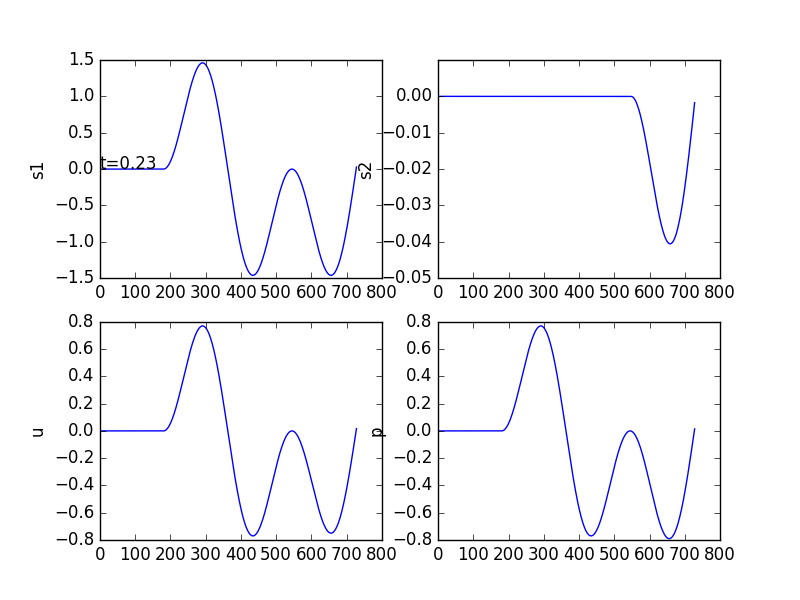
\includegraphics[scale=0.4]{acoustic_eqn_frames/acoustic_eqn_fig05.png}
\centering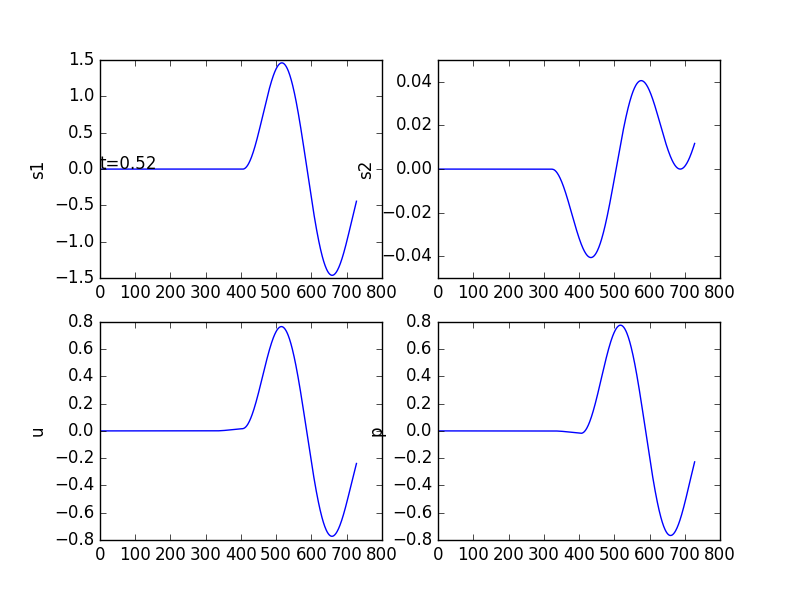
\includegraphics[scale=0.4]{acoustic_eqn_frames/acoustic_eqn_fig10.png}
\centering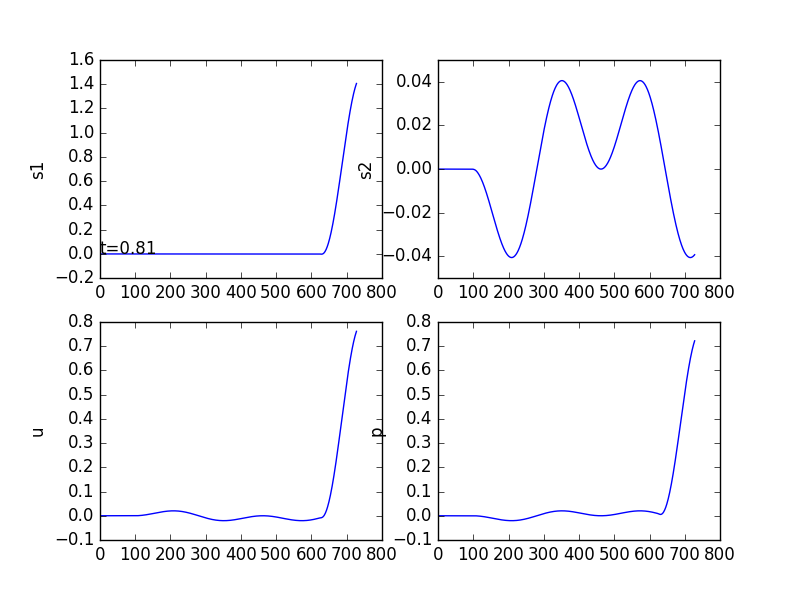
\includegraphics[scale=0.4]{acoustic_eqn_frames/acoustic_eqn_fig15.png}
\caption{Numerical solution for $K=1,$ $\rho=0.9$, $\Delta x = 3^{-6}$, $\Delta t = 0.9 \Delta x / \sqrt{K \rho}$, $p(x,0) = \sin(2\pi x)\sin(4 \pi x),$
$u(x,0) = \sin(2\pi x)\sin(4 \pi x),$.  Top Left 4: $t=0.23$. Top Right 4: $t=0.52$. Bottom 4: $t=0.81$. Top rows: Eigenvector coordinates $s^1$ (right-moving), $s^2$ (left-moving).  Bottom rows: Original coordinates $u,$ $p$.  Shows reflection of data off of right boundary, note the amplitude loss from the original $s^1$ and the reflection, $s^2$.  The data has a peak amplitude of 1.5 in $s^1$ in the first plot, and is reduced to a peak amplitude of 0.04 in $s^2$ in the last plot, but note that the waveform is just a reflection of the original.}
\end{figure}
\begin{figure}[H]

\centering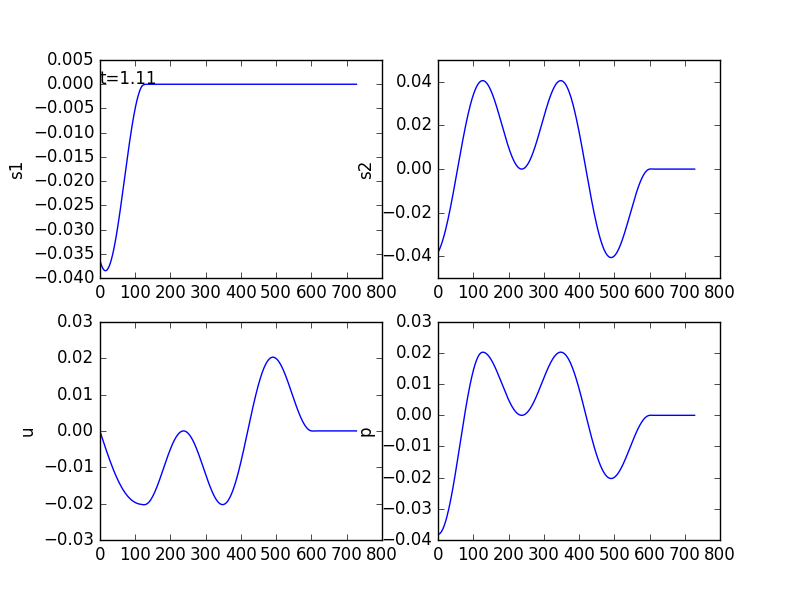
\includegraphics[scale=0.4]{acoustic_eqn_frames/acoustic_eqn_fig20.png}
\centering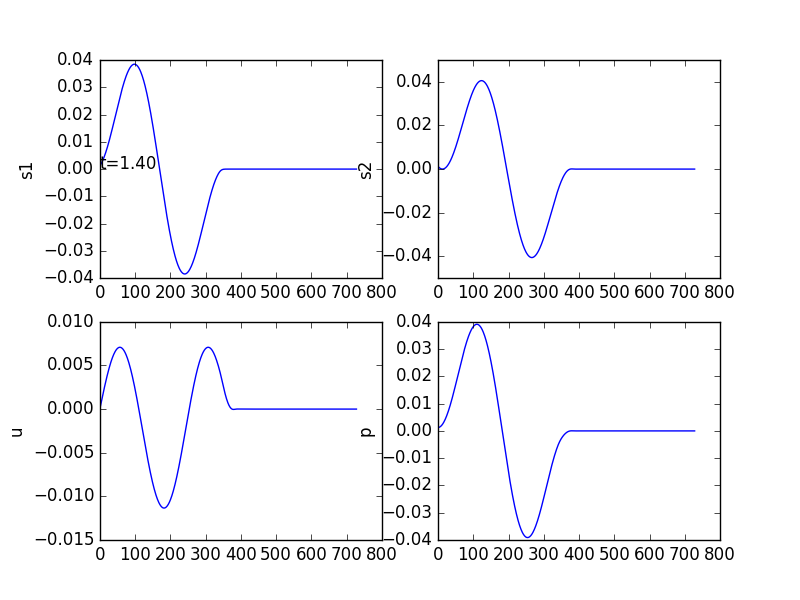
\includegraphics[scale=0.4]{acoustic_eqn_frames/acoustic_eqn_fig25.png}
\centering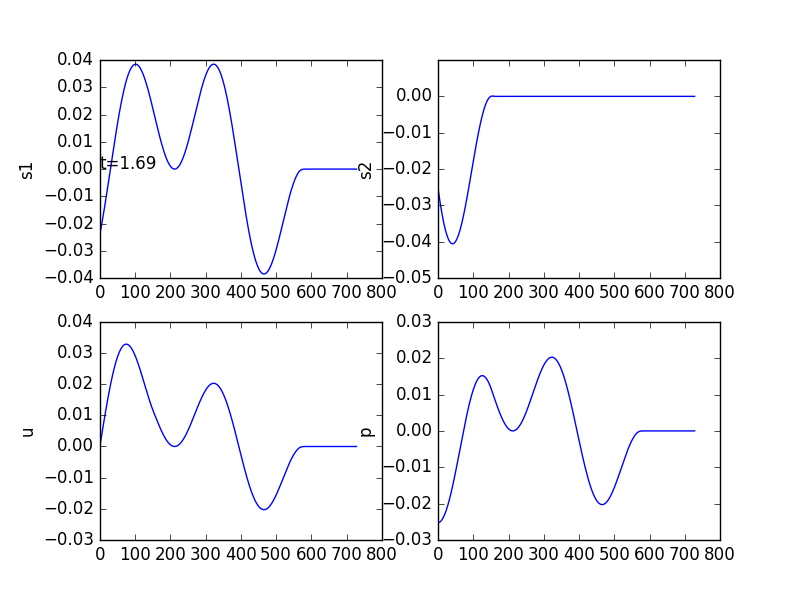
\includegraphics[scale=0.4]{acoustic_eqn_frames/acoustic_eqn_fig30.png}
\caption{Numerical solution for $K=1,$ $\rho=0.9$, $\Delta x = 3^{-6}$, $\Delta t = 0.9 \Delta x / \sqrt{K \rho}$, $p(x,0) = \sin(2\pi x)\sin(4 \pi x),$
$u(x,0) = \sin(2\pi x)\sin(4 \pi x),$.  Top Left 4: $t=1.11$. Top Right 4: $t=1.40$. Bottom 4: $t=1.69$.  Top rows: Eigenvector coordinates $s^1$ (right-moving), $s^2$ (left-moving).  Bottom rows: Original coordinates $u,$ $p$.  Shows reflection of data off of left boundary, note the amplitude conservation from the original $s^2$ and the reflection, $s^1$. The amplitude stays at a peak of 0.04 in both $s^2$ and the reflection $s^1$, and the waveform is just reflected.}
\end{figure}


\item \emph{Give a physical interpretation and a mathematical explanation of these boundary conditions.}


At the left boundary, no flux of ``stuff'' is allowed, i.e., the pressure flux is 0 across the boundary since $p_0^n = p_1^n$, and the velocity is reversed at the boundary since the ``stuff'' is bouncing back.  At the right boundary, a good amount of ``stuff'' is squeezing out the end somehow, but there is also a reflection of a small portion of stuff, so that the waveform is reflected but the amplitudes reduced.   I think we're looking at some sort of flute-like device, with the left boundary capped so nothing can escape, and the right end with a partially capped so that most of the ``stuff'' escapes, but a small amount is reflected back for a kind of resonant effect.
\end{enumerate}
\newpage

%%%%%%%%%%%%%%%%%%%%%%%%%%%%%%%%%%%%%%%%%%%%%%%%%%%%% P2
\begin{myprob}{Problem 2}
Write a program to solve the linear advection equation,
$$u_t + a u_x = 0,$$
on the unit interval using a finite volume method of the form
$$u_j^{n+1} = u_j^n - \dfrac{\Delta t}{\Delta x}\qty(F_{j+1/2} - F_{j-1/2}). $$
Use the numerical flux function
$$F_{j-1/2} = F^{up}_{j-1/2} + \dfrac{|a|}{2}\qty(1-\qty|\dfrac{a\Delta t}{\Delta x}|)\delta_{j-1/2},$$
where $F^{up}_{j-1/2}$ is the upwinding flux,
$$F^{up}_{j-1/2} = \begin{cases}a u_{j-1}, & \text{ if } a>0 \\ 
					a u_{j}, & \text{ if } a<0, \end{cases}$$
and $\delta_{j-1/2}$ is the limited difference.  Let $\Delta u_{j-1/2}=u_j - u_{j-1}$ denote the jump in $u$ across the edge at $x_{j-1/2}$.  The limited difference is 
$$\delta_{j-1/2} \phi(\theta_{j-1/2})\Delta u_{j-1/2}, $$ 
where $$\theta_{j-1/2} = \dfrac{\Delta u_{J_{up}-1/2}}{\Delta u_{j-1/2}}, $$
and $$J_{up} = \begin{cases} j-1, & \text{ if } a>0 \\
							 j+1, & \text{ if } a<0 . \end{cases} $$
Note that you will need two ghost cells on each end of the domain. Write your program so that you may choose from the different limiter functions.

Solve the advection equation with $a = 1$ with periodic boundary conditions for the different initial conditions listed below until time $t = 5$ at Courant number $0.9$.
\begin{enumerate}[(a)]
\item Wave packet: \ \ \ \ \ \ \ \ \ \ \  \ \ \ \ $u(x,0) = \cos(16\pi x)\exp(-50(x-0.5)^2).$
\item Smooth, low frequency: \  \ \ $u(x,0) = \sin(2\pi x)\sin(4 \pi x).$
\item Step function: \ \ \  \ \ \ \ \ \ \  \ \ \ \  $u(x,0) = \begin{cases} 1 & \text{ if } |x-1/2|<1/4 \\ 0 & \text{ otherwise.} \end{cases}$
\end{enumerate}
Compare the results with the exact solution, and comment on the solutions generated by the different methods. How do the different high-resolution methods perform in the different tests? What high-resolution method would you choose to use in practice?
\end{myprob}

I implemented the above finite volume high-resolution methods with variable flux limiter functions.  I used a small time step of $\Delta t = 0.01$ so that the program took an integer number of iterations, $500$ ($5/\Delta t$).  I then used $450$ cell-centered grid points, so that $\nu=a N_x / N_t = 0.9$, and so that the numerical solution could capture the sharp curves at a decent resolution.  Plots of the solutions, for the different flux limiters, against the analytic solution are shown below.  Also given are tables for the 1-norm, 2-norm, and max-norm errors of the various methods (error as compared to the analytic solution).

Figure 3 and Table 3 show the performance of the various methods against the analytic solution for the wave packet initial data.  MC has the smallest error in the 1-norm, 2-norm, and max-norm, so it performs the best on the initial data.  Visually, it doesn't seem to perform much better than the rest, only Upwinding stands out as visibly innacurate.  The wave packet initial data, being smooth and full of various frequencies, is best handled by the middle-of-the-road flux limiter, the MC method.

Figure 4 and Table 4 show the performance of the various methods against the analytic solution for the smooth, low frequency initial data.  MC again has the smallest error in the 1-norm, 2-norm, but Beam-Warming performs better in the max-norm. The other methods (Upwinding aside) have normed errors close to MC's, so MC isn't quite miles ahead of the others.  Visually, it doesn't seem to perform much better than the rest, only Upwinding stands out as visibly innacurate.  The smooth, low frequency initial data is handled almost equally by all but the first-order method.  This isn't surprising, as the smooth, low frequency structure lends itself to easy representation by these 2nd-order methods.

Figure 5 and Table 5 show the performance of the various methods against the analytic solution for the step function initial data.  Superbee has the smallest error in the 1-norm, 2-norm, and max-norm, so it performs by far the best on the initial data.  The difference by which superbee outperforms MC and van Leer here is much more than the amount MC by which outperformed the superbee and van Leer on the other two examples. Visually, it outperforms most of the other methods. LW and BW display high-frequency-phase-lag-induced oscillations near the discontinuities, and Upwinding, minmod, MC, and van Leer show more diffusion than superbee.  The step function initial data, being sharp and discontinuous, is best handled by the most sharpening flux limiter, the Superbee method.

Were I to pick a high-resolution to use in practice, I would go with MC, as it seems the most accurate on general smooth initial data.  However, if I had some insight into my problem and I knew to expect sharp or discontinuous data, I would pick Superbee, as it vastly outperforms MC on that type of data.

\begin{figure}[H]
\centering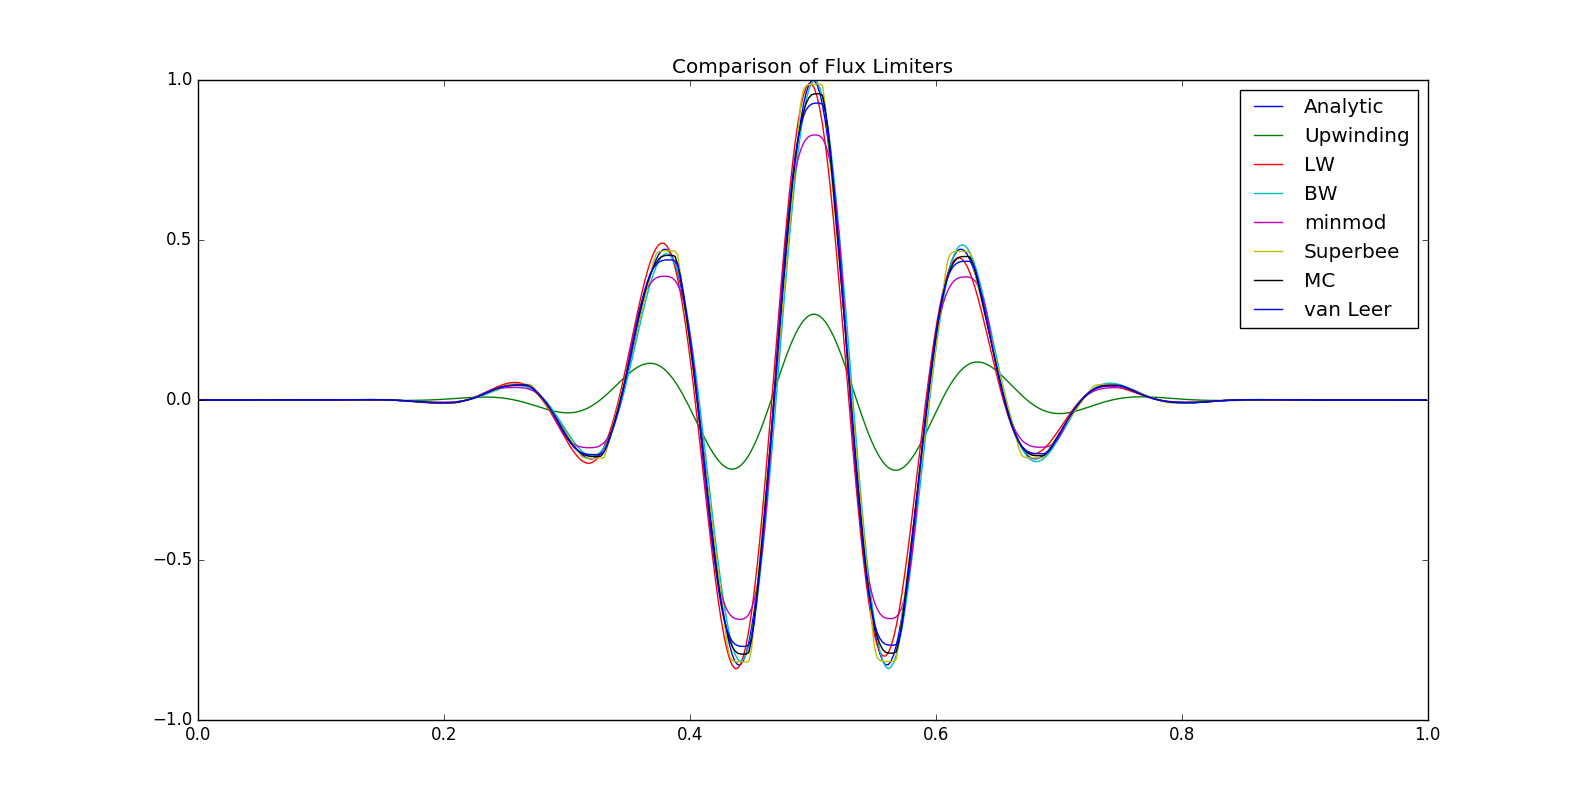
\includegraphics[scale=0.42]{wavepacket_fluxcomp.png}
\caption{Analytic solution vs. numeric for various flux limiters. Wave packet initial data. Numeric parameters: $a=1$, $\Delta t = 0.01$, $\Delta x = 0.01/0.9$ ($N_x = 450$).}
\end{figure}

\begin{table}[H]
\centering\begin{tabular}{||c|l|l|l||}
\hline \hline
   Method &   1-norm error &   2-norm error &   max-norm error \\
\hline
        Upwinding &     0.122216   &      0.222988  &        0.731113  \\
        L-W &     0.018468   &      0.0336219 &        0.106947  \\
        B-W &     0.0107552  &      0.0195931 &        0.0621851 \\
        minmod &     0.0187626  &      0.0385093 &        0.171201  \\
        superbee &     0.0065154  &      0.0131339 &        0.0665255 \\
        \color{red}MC & \color{red}0.00575657 & \color{red}0.0107619 & \color{red}0.0447365 \\
        van Leer &     0.00855164 &      0.0165158 &        0.0736174 \\
\hline \hline
\end{tabular}
\caption{Normed errors for the high-res method solutions compared to the analytic solution. Smooth, low frequency initial data. Numeric parameters: $a=1$, $\Delta t = 0.01$, $\Delta x = 0.01/0.9$ ($N_x = 450$). Note that MC performed the best in all three norms, while superbee and van Leer are performing almost as well.  Note also that Upwinding performs the worst by far in every norm.}
\end{table}

\begin{figure}[H]
\centering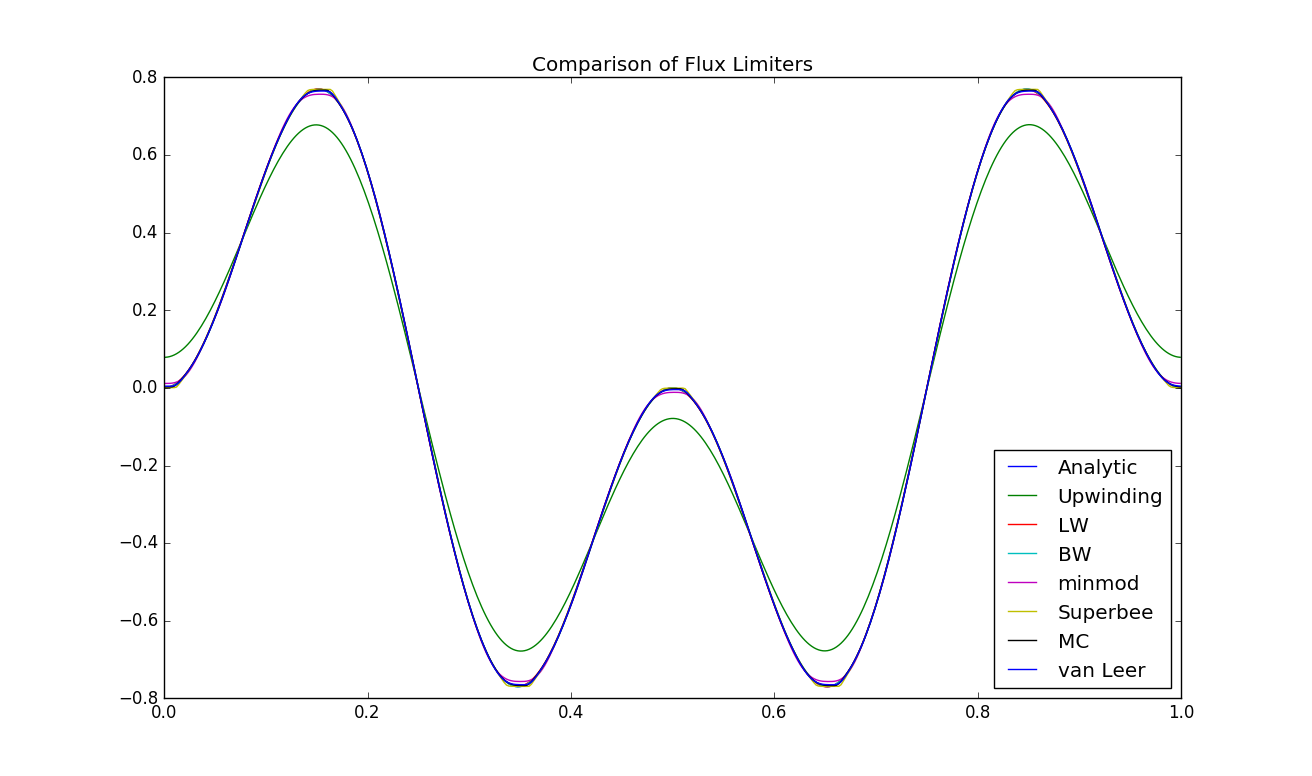
\includegraphics[scale=0.45]{smooth_lowfreq_fluxcomp.png}
\caption{Analytic solution vs. numeric for various flux limiters. Smooth, low frequency initial data. Numeric parameters: $a=1$, $\Delta t = 0.01$, $\Delta x = 0.01/0.9$ ($N_x = 450$).}
\end{figure}

\begin{table}[H]
\centering\begin{tabular}{||c|l|l|l||}
\hline \hline
   Method &   1-norm error &   2-norm error &   max-norm error \\
\hline
        Upwinding &    0.0572338   &     0.0637953  &       0.0950459  \\
        L-W &    0.00166709  &     0.00185234 &       0.00271463 \\
        \color{blue}B-W &    \color{blue}0.000965273 & \color{blue}0.0010725  &       \color{red}0.00157173 \\
        minmod &    0.00310125  &     0.00442548 &       0.0133702  \\
        superbee &    0.00212242  &     0.00292737 &       0.0118801  \\
        \color{red}MC &    \color{red}0.000733134 &  \color{red}0.00105908 & \color{blue}0.00393425 \\
        van Leer &    0.0010299   &     0.00157881 &       0.00527133 \\
\hline \hline
\end{tabular}
\caption{Normed errors for the high-res method solutions compared to the analytic solution. Smooth, low frequency initial data. Numeric parameters: $a=1$, $\Delta t = 0.01$, $\Delta x = 0.01/0.9$ ($N_x = 450$). Note that MC performed the best in the 1 and 2-norms, while B-W performs almost as well, and even better in the max-norm.}
\end{table}

\begin{figure}[H]
\centering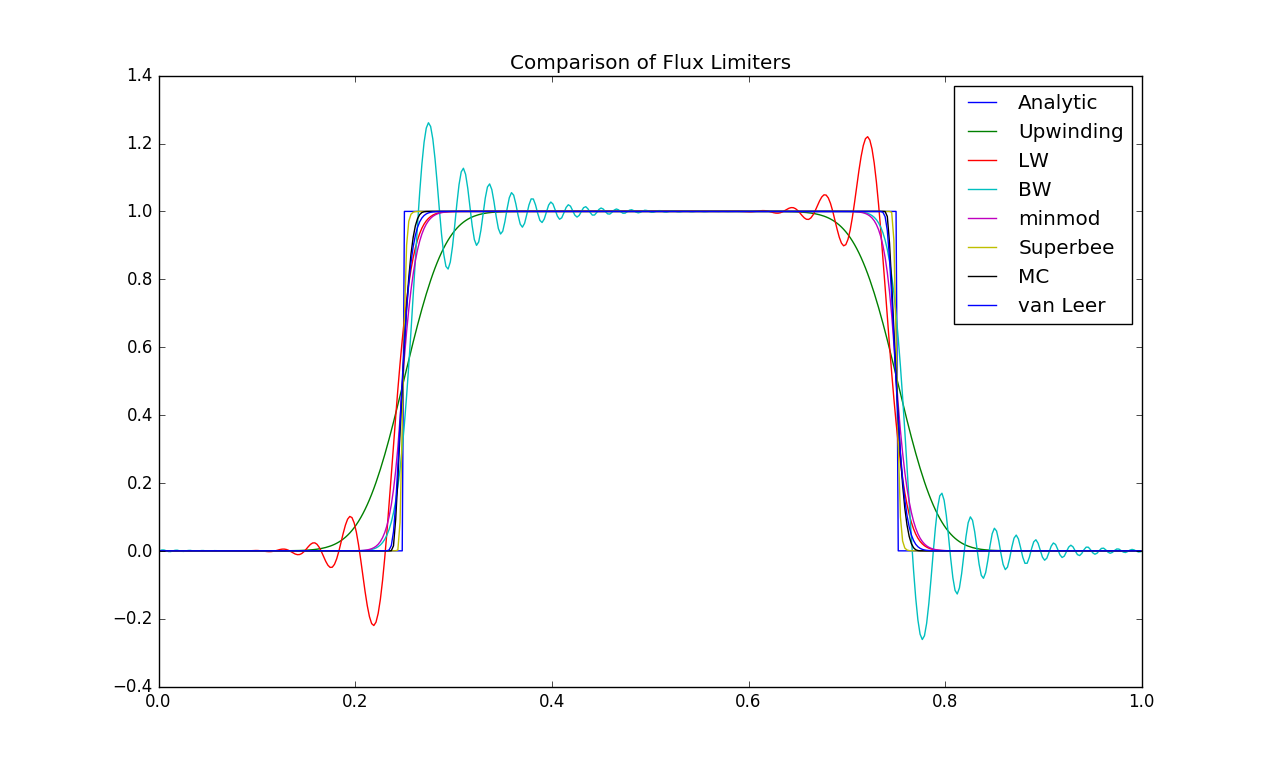
\includegraphics[scale=0.45]{stepfn_fluxcomp.png}
\caption{Analytic solution vs. numeric for various flux limiters. Step function initial data. Numeric parameters: $a=1$, $\Delta t = 0.01$, $\Delta x = 0.01/0.9$ ($N_x = 450$).}
\end{figure}

\begin{table}[H]
\centering\begin{tabular}{||c|l|l|l||}
\hline \hline
   Method &   1-norm error &   2-norm error &   max-norm error \\
\hline
        Upwinding &     0.0531744  &      0.124781  &         0.490248 \\
        L-W &     0.0312041  &      0.0912893 &         0.620986 \\
        B-W &     0.0377079  &      0.0922538 &         0.625865 \\
        minmod &     0.0185625  &      0.0712426 &         0.484127 \\
        \color{red}superbee &  \color{red}0.00409074 &  \color{red}0.0339762 &    \color{red}0.373718 \\
        MC &     0.0102342  &      0.055956  &         0.48307  \\
        van Leer &     0.0118985  &      0.0595052 &         0.501585 \\
\hline\hline
\end{tabular}
\caption{Normed errors for the high-res method solutions compared to the analytic solution. Smooth, low frequency initial data. Numeric parameters: $a=1$, $\Delta t = 0.01$, $\Delta x = 0.01/0.9$ ($N_x = 450$). Note that superbee performs the best in all three norms, while MC and van Leer aren't nearly as accurate.}
\end{table}
\newpage
%===================== CODE ===============================
The following Python code was used for Problem 1.
\begin{verbatim}
def make_diag_fns(K,r):

  def diagonalize(p, u):
    #puts p and u into diagonalized e-vector coordinates s1, s2
    #accepts p and u as row vectors and stacks them in a matrix
    v = np.asarray([p,u])
    Winv = np.asarray([[sqrt(K*r), sqrt(K*r)],[1,-1]])
    return Winv.dot(v)

  def undiagonalize(s):
    #puts e-vector coordinates s1, s2 into original p,u
    W = np.asarray([[1/(2*sqrt(K*r)), 1/2],[1/(2*sqrt(K*r)),-1/2]])
    return W.dot(s)

  return diagonalize, undiagonalize

def LW_matrix(N, nu):
  #set sparse matrix LW for LW method
  #u_j^n+1 = (1-v^2)u_j^n + (v^2-v)/2(u_j+1^n) + (v^2+v)/2(u_j-1^n)
  #on [0,1] ignoring BCs

  #set sub-diagonal components
  sub_diag = (nu**2 +nu)/2*np.ones(N)
  #set above-diagonal components
  above_diag = (nu**2 -nu)/2*np.ones(N)
  #set diagonal components
  diag = (1-nu**2)*np.ones(N)

  # Generate the matrix
  A = np.vstack((sub_diag, diag, above_diag))
  LW = scipy.sparse.dia_matrix((A,[-1,0, 1]),shape=(N,N))
  return LW

def acoustic_LW(u0,p0, LW1, LW2, Nt,K,r):
  #LW method on [0,1] w/ ghost cell BCs for acoustic eqn
  #with time step delT up to time Tf with number of steps Nt=Tf/delT
  #using scheme matrices LW1(delX, nu1), LW2(delX, nu2)

  diagonalize, undiagonalize = make_diag_fns(K,r)
  #start iteration with initial given u0,p0
  #diagonalize
  s_old = diagonalize(p0,u0)

  #setup plots
  plt.axis([0, LW1.shape[0]-2, -2, 2])
  plt.ion()
  frame_no=0
  #do Nt = Tf/delT time steps
  for t in range(Nt):
    #compute ghost cell components
    [p1, u1] = undiagonalize(s_old[:,0])
    # print(p1,u1)
    left_ghost = diagonalize(p1,-u1)
    # print(left_ghost)
    [pN,uN] = undiagonalize(s_old[:,-1])
    right_ghost = diagonalize((1/2)*(pN + uN*sqrt(K*r)),
                  (1/2)*(pN/sqrt(K*r) + uN))
    # print(right_ghost)
    #add ghost cell components
    # print("s=",s_old)
    s_old = np.c_[left_ghost, s_old, right_ghost]
    # print("s=",s_old)
    #advance s w/ LW scheme separately
    s1_old = np.transpose(s_old[0,:])
    s1 = LW1.dot(s1_old)
    # print("s1=",s1)
    s2_old = np.transpose(s_old[1,:])
    s2 = LW2.dot(s2_old)
    # print("s2=",s2)
    #recombine & remove ghost cell components
    s_next = np.r_[[s1[1:-1]],[s2[1:-1]]]
    # print("s=",s_next)

    #update s_old
    s_old = s_next+0

    #plot s, p and u
    if t%50==0:
      [p,u]=undiagonalize(s_old)
      plt.subplot(221); plt.plot(s_old[0]) ;plt.ylabel("s1")
      # plt.axis([0, LW1.shape[0]-2, -2, 2])
      plt.text(0,0,'t=%.4s' % (t*delT))
      plt.subplot(222); plt.plot(s_old[1]); plt.ylabel("s2")
      # plt.axis([0, LW1.shape[0]-2, -2, 2])
      # plt.text(0,0, 'total pressure= %.4s' % (sum(p)))
      plt.subplot(223); plt.plot(u); plt.ylabel("u")
      # plt.axis([0, LW1.shape[0]-2, -2, 2])
      plt.subplot(224); plt.plot(p); plt.ylabel("p")
      # plt.axis([0, LW1.shape[0]-2, -2, 2])
      # plt.text(200,20, 'total velocity= %.4s' % (sum(u)))
      # plt.show(); plt.pause(0.5);
      frame_no=frame_no+1
      if frame_no<10:
        filename='acoustic_eqn_fig0'+str(frame_no)+'.png'
      else:
        filename='acoustic_eqn_fig'+str(frame_no)+'.png'
      savefig(filename)
      plt.close()

  return undiagonalize(s_next)

if __name__ == '__main__':
  #system parameters
  K = 1
  r = 0.9

  #set grid spacings/time steps
  delX = 3**(-6)
  #get time step
  nu1 = 0.9
  #delT = 2**(-10)
  delT = nu1*delX/sqrt(K*r)
  #get grid points for level h
  Nx = int(round(1/delX))
  Nt = 5*int(round(1/delT))
  X = [delX*(j-0.5) for j in range(1,Nx+1)]

  #compute advection/wave speeds
  nu1 = sqrt(K*r)*delT/delX
  print(nu1)
  nu2 = -nu1
  #make LW matrices
  LW1 = LW_matrix(Nx+2,nu1)
  LW2 = LW_matrix(Nx+2,nu2)

  #create initial condition - 0 = Square Pulses, 1= Gaussians, 
  #2=smooth, low freq, 3=wavepacket
  IC = 2
  if IC ==0:
    p0=np.zeros(Nx)
    u0=np.zeros(Nx)
    for j in range(Nx):
      if abs(X[j]-0.5)<=1/4:
        u0[j]=1
        p0[j]=1
  if IC == 1:
    p0 = [exp(-100*(x-0.3)**2) for x in X]
    u0 = [exp(-100*(x-0.8)**2) for x in X]
  if IC==2:
    p0 = [sin(2*pi*x)*sin(4*pi*x) for x in X]
    u0 = [sin(2*pi*x)*sin(4*pi*x) for x in X]
  if IC==3:
    p0 = np.asarray([cos(16*pi*x)*exp(-50*(x-0.5)**2) for x in X])  
    u0 = np.asarray([-cos(16*pi*x)*exp(-50*(x-0.5)**2) for x in X])

  final = acoustic_LW(u0,p0,LW1,LW2,Nt,K,r)

\end{verbatim}

The following Python code was used for Problem 2.
\begin{verbatim}
def make_flux_function(a, delT, delX, phi):
  #constructs numerical flux function using speed a, time step delT, 
  #grid spacing delX, and flux limiter function phi


  def flux(u):
    #compute numerical flux function F_j-1/2 for j=1 to N-1
    Nx = u.shape[0]
    tol = 1e-10
    # print(Nx)
    F = np.zeros(Nx-3)
    # print(F.shape[0])
    for j in range(2,Nx-1):
      #F_j-1/2 = Fup_j-1/2 + |a|/2*(1-|a delT/delX| )*delta_j-1/2
      #with delta_j-1/2 = phi(theta_j-1/2)*(u_j-u_j-1)
      #and theta_j-1/2 = (u_Jup - u_Jup-1)/(u_j - u_j-1)

      #compute Fup_j-1/2 and J_up upwind flux and jump
      if a>=0:
        flux_up = a*u[j-1]
        J_up = j-1
      else:
        flux_up = a*u[j]
        J_up = j+1
      #compute theta_j-1/2 and delta_j-1/2
      denom = u[j] - u[j-1]
      if abs(denom)<=tol:
        delta = 0
      else: 
        theta = (u[J_up] - u[J_up-1])/denom
        delta = phi(theta)*denom
      #compute F_j-1/2
      # print(j-2)
      F[j-2] = flux_up + abs(a)/2*(1-abs(a*delT/delX))*delta
    return F

  return flux

def make_flux_limiter(n):
  #Creates the flux limiter function phi based on the integer n
  #n=0 - Upwinding phi(theta)=0
  if n==0:
    def phi(theta):
      return 0
  #n=1 - Lax-Wendroff phi(theta)=1
  if n==1:
    def phi(theta):
      return 1
  #n=2 - Beam-Warming phi(theta)=theta
  if n==2:
    def phi(theta):
      return theta  
  #n=3 - minmod phi(theta)=minmod(1,theta)
  if n==3:
    def phi(theta):
      return max(0,min(1,theta))
  #n=4 - superbee phi(theta)=max(0,min(1,2theta),min(2,theta))
  if n==4:
    def phi(theta):
      return max(0,min(1,2*theta), min(2,theta))
  #n=5 - MC phi(theta)=max(0,min((1+theta)/2,2,2theta))
  if n==5:
    def phi(theta):
      return max(0,min((1+theta)/2,2,2*theta))
  #n=6 - van Leer phi(theta)=(theta+|theta|)/(1+|theta|)
  if n==6:
    def phi(theta):
      return (theta+abs(theta))/(1+abs(theta))
  return phi    

def high_res_method(u0, flux, delT, delX,Tf, plots_on):
  #High res methods on [0,1] w/ ghost cell periodic BCs
  #with time step delT up to time Tf with number of steps Nt=Tf/delT

  #start iteration with initial given u0
  u_old = u0

  #setup plots
  # plt.figure(1)
  # plt.axis([0, u0.shape[0], -2, 2])
  # plt.ion()
  #do Nt = Tf/delT time steps
  Nt = int(Tf/delT)
  for t in range(1,Nt+1):
    # #compute ghost cell components using periodic BCs
    # left_ghosts = np.r_[u_old[-2],u_old[-1]]
    # right_ghosts = np.r_[u_old[0],u_old[1]]
    # #add ghost cell components
    # u_full = np.r_[left_ghosts, u_old, right_ghosts]
    u_full = np.pad(u_old, (2,2), "wrap")

    #compute flux vectors F_j+1/2, F_j-1/2
    F = flux(u_full)
    F_plus = F[1:]
    F_minus = F[0:-1]

    #compute next u
    u_next = u_old - (delT/delX)*(F_plus-F_minus)

    #update s_old
    u_old = u_next+0

    #plot s, p and u
    if t%20==0 and plots_on==1:
      plt.plot(u_old); plt.ylabel("u")
      plt.axis([0, u0.shape[0], -1, 2])
      plt.text(2,1.8,'t=%.4s' % (t*delT))
      plt.pause(0.5); plt.close()

  return u_old

def main():
  #system parameters
  a=1
  Tf=5

  #set number of grid spacings/time steps
  Nx = 450
  Nt = 500

  #get grid spacing/time step sizes
  delX = 1/Nx
  delT = 1/Nt

  #get courant number
  nu = a*delT/delX
  print(nu)

  #decide whether to plot during simulation
  plots_on = 0

  #IC choice
  IC = 2
  #create initial condition - 0 = wave packet, 
  #  1=smooth,low freq, 2=step function
  X = [delX*(j-0.5) for j in range(1,Nx+1)]
  if IC ==0:
    u0 = np.asarray([cos(16*pi*x)*exp(-50*(x-0.5)**2) for x in X])
  if IC == 1:
    u0 = np.asarray([sin(2*pi*x)*sin(4*pi*x) for x in X])
  if IC==2:
    u0=np.zeros(Nx)
    for j in range(Nx):
      if abs(X[j]-0.5)<=1/4:
        u0[j]=1
  
  final = np.zeros((7, Nx))

  #loop over flux limiters
  for n in range(7):
    #create flux limiter fn phi
    #0 Up, 1 LW, 2 BW, 3 minmod, 4 superbee, 5 MC, 6 van Leer
    phi = make_flux_limiter(n)
    
    #create numerical flux function
    flux = make_flux_function(a,delT,delX,phi)

    final[n] = high_res_method(u0,flux, delT,delX,Tf,plots_on)

  #Compare with analytic solution
  plt.figure(2)
  plt.plot(X, u0)

  #norm-errors
  errors_norm1 = np.zeros(7)
  errors_norm2 = np.zeros(7)
  errors_normmax = np.zeros(7)
  for n in range(7):
    plt.plot(X,final[n])
    #compute norm errors
    error = u0-final[n]
    errors_norm1[n] = delX*sum(abs(error))
    errors_norm2[n] = (delX*sum(error**2))**(1/2)
    errors_normmax[n] = max(abs(error))
  #display errors table
  table = [[i, errors_norm1[i], errors_norm2[i], errors_normmax[i]]
            for i in range(7)]
  print(tabulate(table, headers=["Method", "1-norm error", 
        "2-norm error","max-norm error"], tablefmt="latex"))
  
  plt.title("Comparison of Flux Limiters")

  if IC==1:
    plt.legend(('Analytic', 'Upwinding', 'LW', 'BW', 'minmod', 
      'Superbee', 'MC', 'van Leer'), loc='lower right')
  else:
    plt.legend(('Analytic', 'Upwinding', 'LW', 'BW', 'minmod', 
      'Superbee', 'MC','van Leer'), loc='upper right')
  plt.show()


if __name__ == '__main__':
  main()
\end{verbatim}
\end{document}